\newcommand{\psd}[1]{{\small\sffamily{\color{blue!60}#1}}}




A three-dimensional test synonymous to its two-dimensional counterpart
introduced above is used here as an tutorial example. The problem of
interest is now a unit extrusion (along \(z\)-axis) of the 2D case
above. Cracking is initiated and propagated under tensile loading. The
unit cube with its pre existing crack is clamped at the bottom
\(u_1=u_2=u_3=0\) (first boundary condition) and is loaded
quasi-statically \(u_2=u_2 + \Delta u_2\) on its top surface till the
crack propagates through its walls. So there are two Dirichlet
conditions one on the top border and one on the bottom one.

Just like in the 2D case, to model this test PSD's' hybrid phase-field
modelling technique is used. We will again use ParaView post-processing
of displacement \(u\) and phase-field \(d\) to visualise the cracking
process. A PSD simulation is a two step process, with step one being the
\psd{ PSD\_PreProcess }:

\begin{lstlisting}[style=BashInputStyle]
PSD_PreProcess -dimension 3 -problem damage -model hybrid_phase_field  \
-dirichletconditions 2 -postprocess ud
\end{lstlisting}

Notice that the flags used here are almost similar except for the
\psd{ -dimension 3 } flag, which indeed specifies three-dimensional
problem.

Once the step above has been performed, we solve the problem using four
MPI processes, with the given mesh file \psd{tensile-crack.msh}. This is
step two of the PSD simulation \psd{ PSD\_Solve}.

\begin{lstlisting}[style=BashInputStyle]
PSD_Solve -np 3 Main.edp -mesh ./../Meshes/3D/tensile-crack.msh -v 0
\end{lstlisting}

\begin{figure}[h!]
\centering

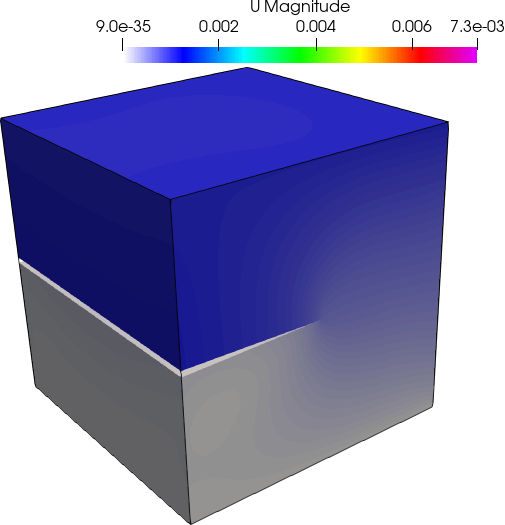
\includegraphics[width=0.24\textwidth]{./Images/u3d0.png}
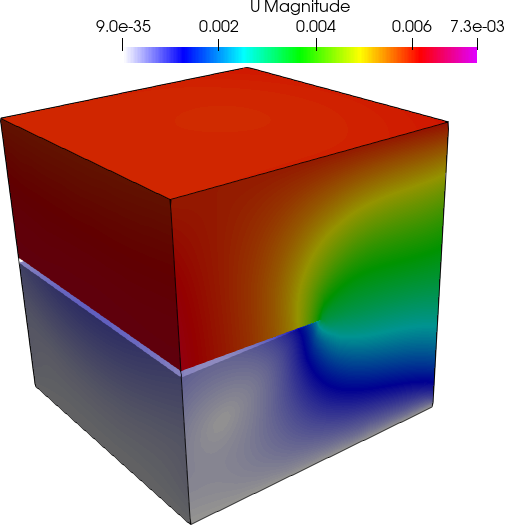
\includegraphics[width=0.24\textwidth]{./Images/u3d1.png}
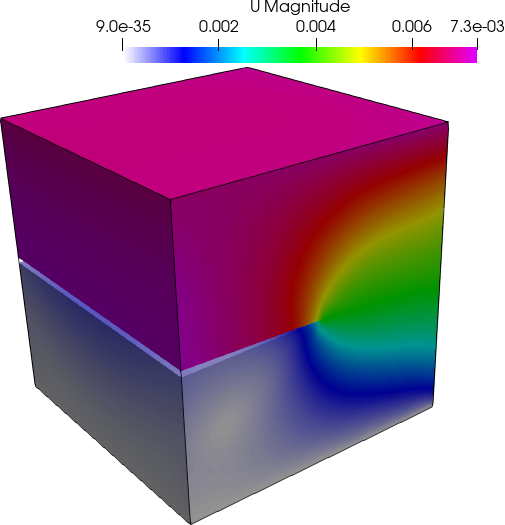
\includegraphics[width=0.24\textwidth]{./Images/u3d2.png}
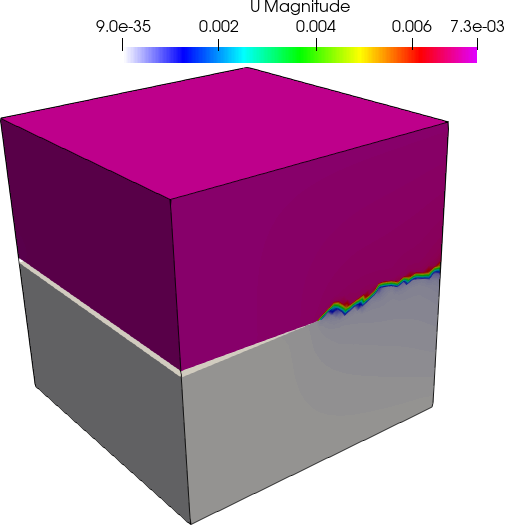
\includegraphics[width=0.24\textwidth]{./Images/u3d3.png}
\caption{Finite element displacement visualised for the 3D problem with ParaView at different timesteps (quasi-statics). Time progresses from left to right in a row and top to bottom when comparing rows. \label{u3d-fem}}
\end{figure}

\begin{figure}[h!]
\centering

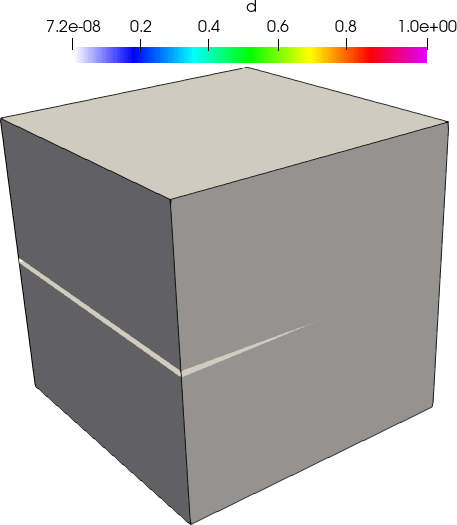
\includegraphics[width=0.24\textwidth]{./Images/d3d0.png}
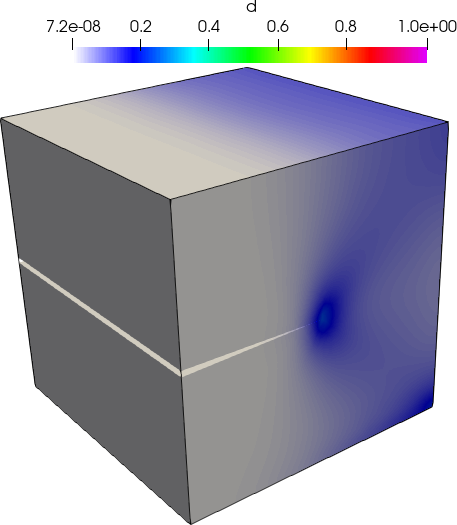
\includegraphics[width=0.24\textwidth]{./Images/d3d1.png}
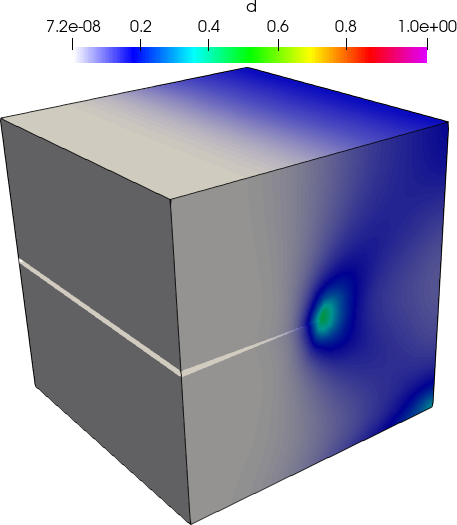
\includegraphics[width=0.24\textwidth]{./Images/d3d2.png}
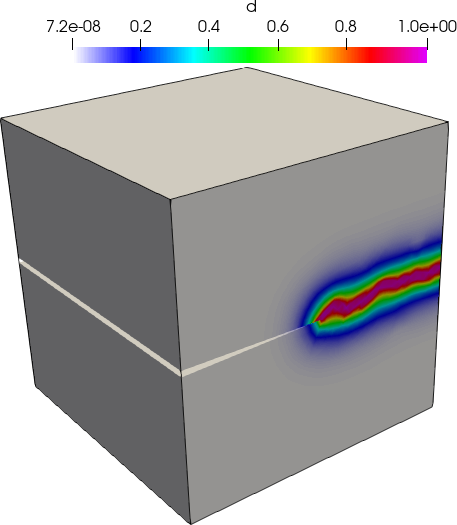
\includegraphics[width=0.24\textwidth]{./Images/d3d3.png}
\caption{Finite element damage visualised for the 3D problem with ParaView at different timesteps (quasi-statics). Time progresses from left to right in a row and top to bottom when comparing rows. \label{d3d-fem}}
\end{figure}

Figures \ref{u3d-fem} and \ref{d3d-fem} present the finite element
displacement and damage field of the 3D problem, which enable us to
visualise the cracking of the cubic specimen.
